\documentclass[12pt]{article}

\usepackage{sbc-template}

\usepackage{graphicx,url}

\usepackage[utf8]{inputenc}

\sloppy

\title{Groovy on Rails, uma alternativa para o desenvolvimento de aplicações web sem sair da Plataforma Java}

\author{Marcelo Emanoel Bezerra Diniz\inst{1}}

\address{
    Centro de Ciências Tecnológicas -- Universidade de Fortaleza (UNIFOR)\\
    CEP 60.811-905 -- Fortaleza -- CE -- Brasil
}

\begin{document} 

\maketitle

\begin{resumo} 
    Desde seu surgimento a plataforma Java se destaca como uma ótima alternativa para o desenvolvimento de aplicações web.
    Diversos frameworks surgiram para proporcionar reutilização de código e aumento de produtividade. A plataforma possui 
    implementações robustas e amplamente utilizadas. Porém, apesar dos esforços, outras tecnologias mais recentes vem se 
    destacando e tomando a frente no cenário de desenvolvimento de aplicações para a web. Dentre estas tecnologias são notórias
    algumas características como o uso de linguagens dinâmicas em conjunto com padrões de projeto amplamente conhecidos.
    Neste artigo será abordado o framework Groovy on Rails, ou simplesmente, Grails. O framework alia a linguagem dinâmica groovy
    à arquitetura utilizada no Ruby on Rails. 
\end{resumo}

\section{Introdução}
    Alta competitividade, baixo custo de produção e manutenção além de alta qualidade são exigências do mercado de desenvolvimento
    de software. Independentemente da tecnologia envolvida no processo de construção de uma aplicação web, existe o componente de 
    complexidade inerente ao próprio ambiente. Toda a comunicação é baseada no protocolo HTTP. Sua simplicidade garante a alta 
    disponibilidade da Web, porém requer um trabalho adicional das aplicações para manter as informações seguras e íntegras.

    No cenário previamente descrito a Plataforma Java se destacou desde o seu surgimento. A fim de facilitar o desenvolvimento
    das aplicações para este ambiente, surgiram diversos frameworks, bases de infra-estruturas extensíveis, voltadas para um nicho
    em particular. A partir destas o desenvolvedor irá retirar os insumos para a construção de aplicações.

    Com o passar do tempo outras linguagens dentro e fora da plataforma foram surgindo com propostas um pouco diferentes da linguagem
    Java. Algumas com características funcionais outras com características totalmente orientadas a objetos. Porém todas com um foco 
    em comum, aumento de produtividade, possibilitando entregar mais funcionalidades com menos código. Em cima dessas novas linguagens
    novos frameworks foram sendo desenvolvidos para resolver de forma melhor os antigos problemas.
    
    Nesse cenário, por volta do ano de 2006, surgiu o framework Ruby on Rails para a linguagem Ruby. Suas bases advêm do padrão de
    projeto MVC. Voltado para o desenvolvimento de aplicações web, rapidamente adquiriu adeptos por facilitar e agilizar a criação 
    de aplicações através de geradores de código para as tarefas comuns além é claro da utilização de uma linguagem de mais fácil
    compreensão.

    Com a popularização desse conjunto de novas linguagens, implementações baseadas na Java Virtual Machine foram surgindo e através 
    da JSR 223, a integração de linguagens de script foi facilitada. Nesse contexto uma nova linguagem surgiu, Groovy. Criada especificamente
    para utilização na JVM propicia a possibilidade de inovação que a tanto a linguagem Java necessita. Além disso, alia o extenso 
    conjunto de bibliotecas Java pré-existentes às facilidades da nova linguagem de maneira transparente. 
    
    Com a popularização do Ruby on Rails muitas de suas funcionalidades passaram foram incorporadas por alguns frameworks mesmo que em 
    outras linguagens. A abordagem utilizada no Groovy on Rails, Grails, possui algumas similaridades e algumas diferenças. Seu foco está
    em utilizar fórmulas consagradas na Plataforma Java e aliar às inovações do Rails produzindo um ambiente de alta produtividade utilizando
    soluções maduras.
    
    Nas seções seguintes serão descritos os principais conceitos da linguagem Groovy e do framework Grails.

\section{First Page} \label{sec:firstpage}

The first page must display the paper title, the name and address of the
authors, the abstract in English and ``resumo'' in Portuguese (``resumos'' are
required only for papers written in Portuguese). The title must be centered
over the whole page, in 16 point boldface font and with 12 points of space
before itself. Author names must be centered in 12 point font, bold, all of
them disposed in the same line, separated by commas and with 12 points of
space after the title. Addresses must be centered in 12 point font, also with
12 points of space after the authors' names. E-mail addresses should be
written using font Courier New, 10 point nominal size, with 6 points of space
before and 6 points of space after.

The abstract and ``resumo'' (if is the case) must be in 12 point Times font,
indented 0.8cm on both sides. The word \textbf{Abstract} and \textbf{Resumo},
should be written in boldface and must precede the text.

\section{CD-ROMs and Printed Proceedings}

In some conferences, the papers are published on CD-ROM while only the
abstract is published in the printed Proceedings. In this case, authors are
invited to prepare two final versions of the paper. One, complete, to be
published on the CD and the other, containing only the first page, with
abstract and ``resumo'' (for papers in Portuguese).

\section{Sections and Paragraphs}

Section titles must be in boldface, 13pt, flush left. There should be an extra
12 pt of space before each title. Section numbering is optional. The first
paragraph of each section should not be indented, while the first lines of
subsequent paragraphs should be indented by 1.27 cm.

\subsection{Subsections}

The subsection titles must be in boldface, 12pt, flush left.

\section{Figures and Captions}\label{sec:figs}


Figure and table captions should be centered if less than one line
(Figure~\ref{fig:exampleFig1}), otherwise justified and indented by 0.8cm on
both margins, as shown in Figure~\ref{fig:exampleFig2}. The caption font must
be Helvetica, 10 point, boldface, with 6 points of space before and after each
caption.

\begin{figure}[ht]
\centering
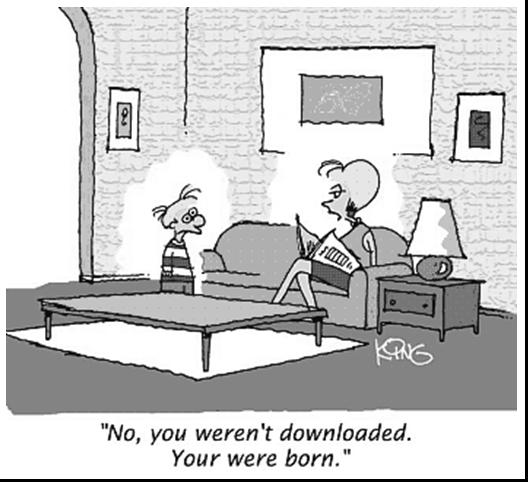
\includegraphics[width=.5\textwidth]{fig1.jpg}
\caption{A typical figure}
\label{fig:exampleFig1}
\end{figure}

\begin{figure}[ht]
\centering
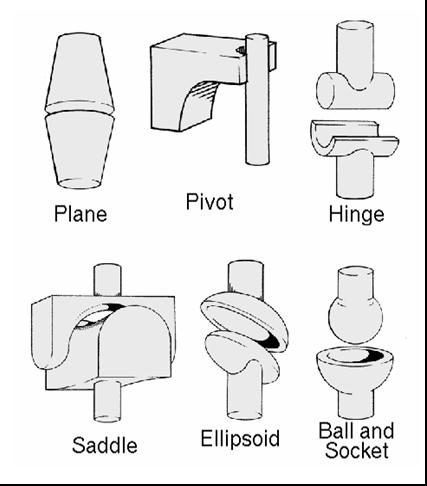
\includegraphics[width=.3\textwidth]{fig2.jpg}
\caption{This figure is an example of a figure caption taking more than one
  line and justified considering margins mentioned in Section~\ref{sec:figs}.}
\label{fig:exampleFig2}
\end{figure}

In tables, try to avoid the use of colored or shaded backgrounds, and avoid
thick, doubled, or unnecessary framing lines. When reporting empirical data,
do not use more decimal digits than warranted by their precision and
reproducibility. Table caption must be placed before the table (see Table 1)
and the font used must also be Helvetica, 10 point, boldface, with 6 points of
space before and after each caption.

\begin{table}[ht]
\centering
\caption{Variables to be considered on the evaluation of interaction
  techniques}
\label{tab:exTable1}
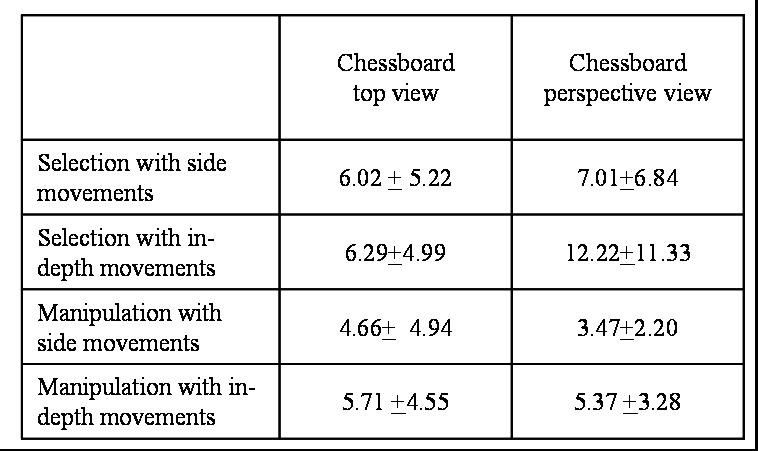
\includegraphics[width=.7\textwidth]{table.jpg}
\end{table}

\section{Images}

All images and illustrations should be in black-and-white, or gray tones,
excepting for the papers that will be electronically available (on CD-ROMs,
internet, etc.). The image resolution on paper should be about 600 dpi for
black-and-white images, and 150-300 dpi for grayscale images.  Do not include
images with excessive resolution, as they may take hours to print, without any
visible difference in the result. 

\section{References}

Bibliographic references must be unambiguous and uniform.  We recommend giving
the author names references in brackets, e.g. \cite{knuth:84},
\cite{boulic:91}, and \cite{smith:99}.

The references must be listed using 12 point font size, with 6 points of space
before each reference. The first line of each reference should not be
indented, while the subsequent should be indented by 0.5 cm.

\bibliographystyle{sbc}
\bibliography{sbc-template}

\end{document}
